\section{Preliminaries} \label{sec:preliminary}
This section aims to cover background on gradient clipping in DP optimization and explain why alternate group-wise clipping strategies can be attractive from a computational efficiency standpoint.

Our work trains machine learning models (more precisely deep neural networks) with optimizers that guarantee $(\epsilon, \delta)$-DP.
In our case, $\M$ is an optimization algorithm which outputs the learned model parameters $\vtheta$. 
Widely used DP optimizers (e.g., DP-SGD) usually introduce two additional steps before each parameter update to privatize gradients:
(1) clip per-example gradients of a minibatch by their Euclidean norms according to some threshold $C$;
(2) add Gaussian noise to the sum of clipped gradients. 
In practice, the clipping threshold $C$ can be either a tunable hyperparameter or set to some (privatized) statistic estimated from data. 
The standard deviation of the Gaussian noise is determined by the clipping threshold $C$ and the noise multiplier $\sigma$, the latter of which is set by a privacy accounting procedure given target privacy parameters $(\epsilon, \delta)$, the number of iterations $T$, and the subsampling rate $\rho$~\citep{abadi2016deep,mironov2017renyi, dong2019gaussian, gopi2021numerical}. 
We now present background on different per-example gradient clipping strategies in DP optimization.

\textbf{Flat Clipping.}
This is the clipping scheme used in the original DP-SGD algorithm~\citep{abadi2016deep}.
Here, the gradient of example $s_i$'s loss $\ell(\vtheta, s_i)$ with respect to model parameters $\vg^{(i)}:= {\partial \ell(\vtheta, s_i)} / {\partial \vtheta}$ is normalized if its magnitude exceeds the threshold $C$.
Thus, the actual contribution (up to scaling) of the $i$th instance to the noisy gradient is
$\widetilde{\vg}^{(i)} := \vg^{(i)}\cdot \min \{1, C /  {\|\vg^{(i)}\| } \}$.
Flat clipping cannot be performed until the gradient norms $\{\|\vg^{(i)}\|\}_i$ are computed. 
Since the latter quantities are only known after backpropagation completes, flat clipping necessitates a second-round of computation after backpropagation to conditionally rescale the gradients. 
This is a source of overhead and presents complications when model weights don't fit on a single device. 



\textbf{Group-Wise Clipping.} 
This scheme partitions the set of parameters $\vtheta \in \R^d$ into $K$ disjoint groups $\{\vtheta_k  \}_{k=1}^K$ with  $\vtheta_k \in \sR^{d_k}$ for $k\in [K]$.
For each group $k$, the scheme prescribes a clipping threshold $C_k$. 
Denote example $s_i$'s gradient for the $k$th group by $\vg_k^{(i)}:= {\partial \ell(\vtheta, s_i)} / {\partial \vtheta_k}$.
Under group-wise clipping, the $k$th clipped gradient for $s_i$ is 
$\tilde{\vg}_k^{(i)} := \vg_k^{(i)}\cdot \min\{1, C_k / {\|\vg_k^{(i)}\|}\}$.
Next, we present two instantiations of group-wise clipping that are computationally advantageous in different settings.









\section[Efficient Private Learning with Adaptive Per-layer Clipping]{Efficient Private Learning with \\Adaptive Per-layer Clipping} \label{sec:benefit-loss}
The first instantiation of group-wise clipping we study is per-layer clipping which clips gradients of separate neural network layers separately.
This scheme had been presented in past works~\citep{mcmahan2018general,mcmahan2018learning,dupuy2022efficient},
but neither its computational properties nor its performance implications had been carefully studied.
We show that with proper implementation, per-layer clipping can be as memory-efficient and almost as time-efficient as non-private training for small- to moderate-scale workflows that run on single accelerators.
Additionally, we confirm that per-layer clipping with hand-set thresholds underperforms flat clipping and demonstrate that adaptively setting these thresholds eliminates potential performance losses. 


\subsection[Per-layer Clipping DP-SGD Can Be Almost as Efficient as Non-private SGD]{Per-layer Clipping DP-SGD Can Be as Efficient as SGD}
Per-layer clipping groups together parameters of a neural network layer (e.g., linear, convolution) and prescribes each of the $K$ layers of the network a clipping threshold $C_k$ to clip the gradient of that layer. This directly implies that gradient clipping for any layer can be performed as soon as backpropagation reaches that layer (to construct per-example gradients or norms) when parameter sharing is absent, and is unlike flat clipping which cannot be performed until backpropagation completes entirely.\footnote{Note the DP learning library Opacus~\citep{yousefpour2021opacus} has a per-layer clipping optimizer which supports clipping each layer with a separate threshold. But this implementation conducts per-layer clipping after backpropagation completes and instantiates all per-example gradients before clipping, which is inefficient.
}

Our efficient implementation of per-layer clipping clips layer-wise gradients as soon as the gradient with respect to outputs of that layer are returned from backpropagation.
The operations of clipping and summing per-example gradients can be fused once input activations, output gradients, and per-example gradient norms are known. In addition, per-example gradient norms can be cheaply computed without materializing actual per-example gradients in memory~\citep[Section 4]{li2022large}.
This implementation results in private training that is as memory-efficient as non-private training since per-example gradients are not instantiated, and almost as time-efficient per update since the extra computation involving gradient norm and gradient scaling are typically cheap.
Figure~\ref{fig:throughput-comparison} shows that carefully implemented per-layer clipping matches the memory profile and almost matches the training throughput of non-private learning for an autoregressive fine-tuning task with GPT-2 on a single GPU (we followed the same experimental protocol as that of Section 4 in~\citep{li2022large} for a fair comparison).
See Appendix~\ref{app:runtime} for additional experiments with head-to-head wall time comparisons. 

\begin{figure}[htb]
\begin{center}
\begin{minipage}[t]{0.48\linewidth}
\centering
{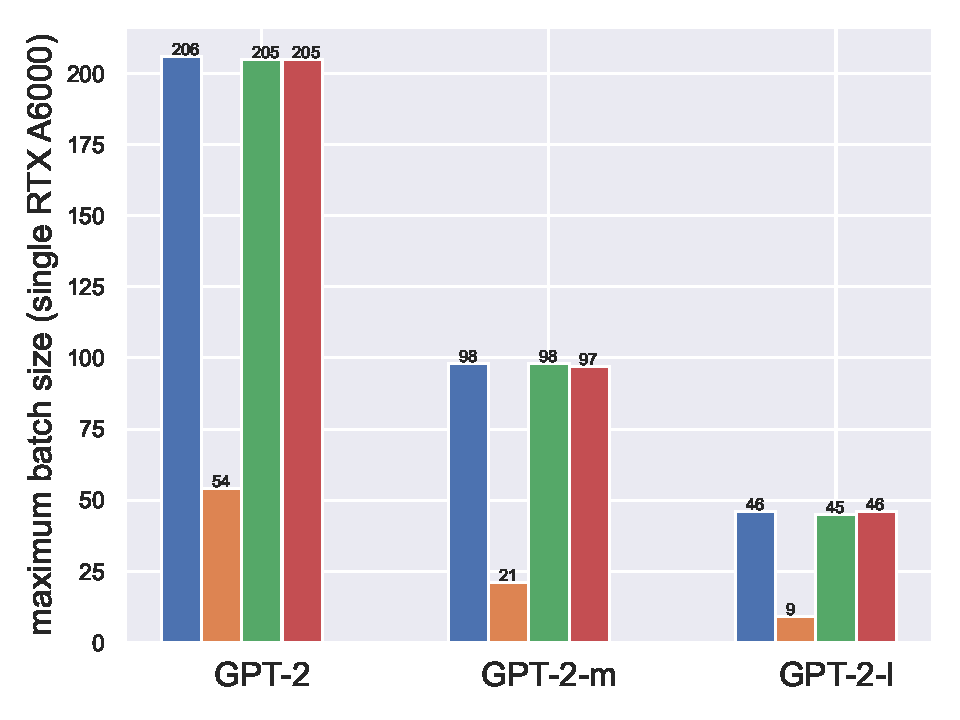
\includegraphics[width=0.9\linewidth]{files/fig/memory_100_default_fast_float.pdf}} \\
(a) Memory
\end{minipage}
\begin{minipage}[t]{0.48\linewidth}
\centering
{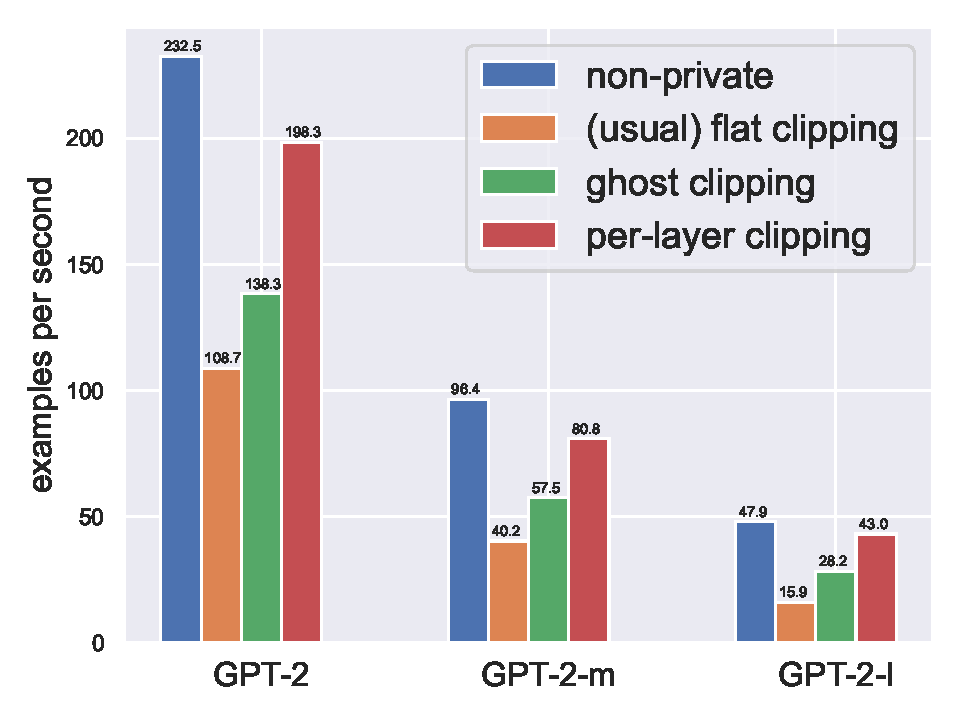
\includegraphics[width=0.9\textwidth]{files/fig/throughput_100_default_fast_float.pdf}} \\
(b) Throughput
\end{minipage}
\end{center}
\caption{
Private learning with (adaptive) per-layer clipping can be almost as efficient as non-private learning (the throughput gap is less than 15\% in this case).
Here, ``(usual) flat clipping'' refers to the implementation which first creates and stores in memory all per-example gradients (e.g., adopted in Opacus~\citep{yousefpour2021opacus}).
Ghost clipping~\citep{li2022large} is based on flat clipping but avoids materializing per-example gradients by performing an additional backward pass each time. 
}
\label{fig:throughput-comparison}
\end{figure}







\subsection{(Fixed) Per-layer Clipping May Hurt the Utility}

Despite the computational advantages, per-layer clipping with fixed clipping thresholds set by hand (which we refer to as \emph{fixed per-layer clipping}) reportedly underperforms flat clipping \citep{mcmahan2018learning}. 
To further verify this and remove confounding effects of potentially suboptimal hyperparameters, we compare fixed per-layer clipping against (fixed) flat clipping on two tasks: 
1) training wide ResNet (WRN16-4) \citep{zagoruyko2016wide} from scratch to classify CIFAR-10 images, and
2) fine-tuning the pretrained RoBERTa-base for classifying sentiment on SST-2. 
% We carefully tuned the clipping thresholds and learning rate for both clipping methods; see Appendix \ref{app:hyperparameter} for details.
We carefully tuned the clipping thresholds and learning rate for both clipping methods.
Tables~\ref{table:fixed_global_cifar10} and \ref{table:fixed_global_sst2} confirm that per-layer clipping with hand-set fixed thresholds underperforms flat clipping. 
\begin{table}[h]
\footnotesize
\setlength\tabcolsep{2.4pt}
\caption{Fixed per-layer clipping underperforms (fixed) flat clipping.
}
\label{table:fixed_global}

\begin{subtable}[h]{0.45\textwidth}
\centering
\caption{CIFAR-10 validation accuracy over  3 seeds.} %
\begin{tabular}{l l ccc ccc}
\toprule
{Model} &
{Method} & 
\text{$\epsilon=3$} & 
\text{$\epsilon=8$} \\
\midrule
\multirow{2}{*}{WRN16-4} 
& Fixed per-layer & 60.6 & 67.8 \\ %
& Fixed flat & 63.1 & 73.9 \\
\bottomrule
\end{tabular}
\label{table:fixed_global_cifar10}
\end{subtable}
\hfill
\begin{subtable}[h]{0.45\textwidth}
\centering
\caption{SST-2 validation accuracy over 3 seeds.} %
\label{table:fixed_global_sst2}
\begin{tabular}{l l ccc ccc}
\toprule
{Model} &
{Method} & 
\text{$\epsilon=3$} & 
\text{$\epsilon=8$} \\
\midrule
\multirow{2}{*}{RoBERTa-base} 
& Fixed per-layer & 89.4 & 89.7 \\ %
& Fixed flat & 91.0 & 91.7 \\
\bottomrule
\end{tabular}

\end{subtable}
\end{table}







To understand why fixed per-layer clipping gives worse performance, we plot the per-layer gradient norms of randomly sampled CIFAR-10 examples for privately training WRN16-4 in Figure \ref{fig:grad-norm-cifar10}.
 % (see Appendix \ref{app:gradnorm-shift} for the setup). 
We observe that the general magnitudes of per-layer gradient norms change dramatically across training. 
Early on, gradient norms are generally uniformly low across all layers. 
As training proceeds, gradient norms for layers close to the input gradually become high. 
% We present additional evidence for this phenomenon with language model fine-tuning in Appendix~\ref{app:gradnorm-shift}. 

These observations suggest that clipping with fixed layer-wise thresholds likely removes the structural relation between gradients of different layers. 
This incurs an extra source of bias in addition to the usual bias of flat clipping that alters the relation of gradients across samples and makes balancing clipping bias and privacy noise throughout training more challenging. 
These observations motivate us to set the thresholds based on some adaptively estimated statistic of layer-wise gradients. 

\begin{figure}[ht]
\centering
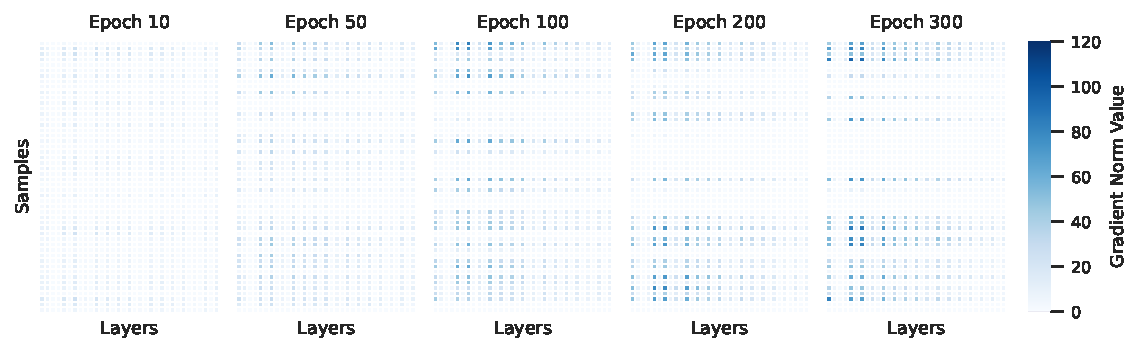
\includegraphics[width=0.85\textwidth]{files/fig/persample_perlayer_norm_cifar.pdf}
\caption{The distribution of per-layer gradient norms shifts substantially across training. Each column represents one layer, and each row represents one example. 
Layers of the neural network are placed from input (left) to output (right). 
Darker colors indicate higher values of gradient norms. 
}
\label{fig:grad-norm-cifar10}
\end{figure}

\subsection{Adaptive Per-layer Clipping Can Be \\as Effective as Flat Clipping}
\label{sec:adaptive-clipping}

\begin{wrapfigure}[13]{R}{0.45\textwidth}
    \centering
    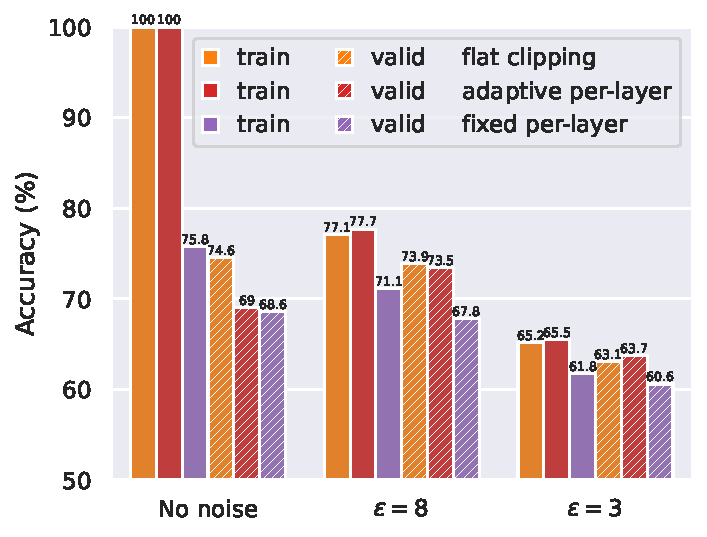
\includegraphics[width=.38\textwidth]{files/fig/cifar_withour_noise_single.pdf}
    \caption{Adaptive per-layer clipping eliminates performance losses experienced by fixed per-layer clipping.}
    \label{fig:cifar_without_noise}
\end{wrapfigure}
To overcome the above performance issues of fixed per-layer clipping, we consider per-layer clipping with adaptive clipping thresholds that we herein refer to as \emph{adaptive per-layer clipping}. 
Our hope is that the adaptive thresholds can track gradient norm shift, capture gradient structure, and consequently mitigate the structural bias caused by clipping gradients of separate layers separately. 
One candidate statistic for setting the adaptive threshold is some quantile of gradient norms. 
Notably, \cite{andrew2019differentially} provided an effective way of estimating  quantiles privately for flat clipping via online convex optimization.
We adapt their algorithm to the per-layer setup and let each layer maintain an online estimate of a target gradient norm quantile. %


Two questions arise with this formulation: 1) How should the per-layer gradient norm quantiles be privately estimated, and 2) how should the noise levels for different layers be decided? 
We address the two questions below. 
Algorithm \ref{alg:perlayer-DPSGD} delineates the overall procedure in pseudocode, where per-layer gradient clipping in conjunction with backpropagation occurs on lines 7-12, adaptive private quantile estimation occurs on lines 15-18, and noise allocation occurs on line 13. 
The pseudocode is based on DP-SGD, but its core ideas naturally apply to private versions of other first-order optimizers (e.g., DP-Adam).



\paragraph{Estimating quantiles privately.}
We allocate some privacy budget (in practice $r=$1\% to 10\% of total budget) to estimate a target quantile of each layer's gradient norms. 
Clipping thresholds $C_1, ..., C_K$ are then set to these estimated quantiles. 
We record the number of gradients clipped before each parameter update and adjust the clipping threshold based on whether too many or too few are clipped. 
The central quantity which needs to be privatized is then the fraction of clipped gradients.
We introduce the additional noise multiplier $\sigma_{b}$ to privatize this fraction statistic (used in Gaussian mechanism). 
The new noise multiplier $\sigma_\text{new}$ (based on $1-r$ fraction of total budget) for noising parameter updates is computed with the following proposition.
% , whose proof we defer to Appendix~\ref{app:proofs}.


\begin{prop}\label{prop:noise-multiplier}
Let $\sigma$ be the original noise multiplier for noising parameter updates to achieve a certain level of differential privacy (without private quantile estimation) and $\sigma_b$ be chosen for noising quantile estimates (release of the latter consumes $r$ fraction of the privacy budget). %
Then the new noise multiplier $\sigma_{\text{new}}$ for noising parameter updates (consuming $1-r$ fraction of the budget) is
\begin{equation}
\sigma_{\text{new}} = (\sigma^{-2}- K/(2\sigma_b)^2)^{-1/2}. \label{eq:sigma_new_sigma_b}    
\end{equation}
\end{prop}

\begin{proof}
The proof is based on direct calculation, a simple version of which is given in \cite{andrew2019differentially}. First, we note that the clip counts $b_k^{(i)}$ is either 0 or 1 (see line 10 in Algorithm \ref{alg:perlayer-DPSGD}). One can make it to be symmetric by using $b_k^{(i)} -\frac{1}{2}$, whose sensitivity is $\frac{1}{2}$. Suppose the gradient has sensitivity $S$. 

For the Gaussian mechanism, to keep the privacy budget constant we have 
\begin{flalign*}
S^2/(S\sigma)^2 = S^2/(S\sigma_{\text{new}})^2 + K\cdot \frac{(1/2)^2}{\sigma_b^2}.
\end{flalign*}
Simplifying the above expression, we get $\sigma_{\text{new}}$.


We can further compute the fraction $r$ of budget that is used to privately estimate quantiles by  
$r=K\cdot \frac{(1/2)^2}{\sigma_b^2}/(1/\sigma^2)$. We can also derive the value of $\sigma_b$ given $r$ from the above formula.
\end{proof}

\begin{Remark}
The private quantile estimation for $K$ groups costs a fraction $r = K\sigma^2/(4\sigma_b^2)$ of privacy budget (in terms of R\'enyi differential privacy~\citep{mironov2017renyi}). 
\end{Remark}

\paragraph{Allocating noise.}
The original Gaussian mechanism adds isotropic noise to statistics before their release~\citep{dwork2014algorithmic} which results in different coordinates experiencing the same amount of noise.
Yet, simply scaling different components with public quantities (before adding noise) allows different components to experience different levels of noise. 
As an example, let $\gamma_1, \cdots, \gamma_K$ be coefficients for scaling, and recall that $\tilde{\vg}_k$ is the sum of clipped gradients for layer / group $k$. 
Then, applying the Gaussian mechanism to the scaled $\hat{\vg} := (\hat{\vg}_1, ..., \hat{\vg}_K)$, where $\hat{\vg}_k:={\tilde{\vg}_k}/{\gamma_k}$, and rescaling back the privatized quantities afterwards ends up adding noise to $\tilde{\vg}_k$ that has standard deviation proportional to $\gamma_k$.

Among the possible ways of choosing $\{\gamma_1, ..., \gamma_K\}$, we outline two simple approaches that we found to be effective for different reasons in our empirical studies. We use the global strategy in all but experiments with GPT-3.
% Appendix~\ref{app:noise-allocation} includes empirical studies of alternate strategies.
\begin{itemize}[leftmargin=6mm,noitemsep]
    \item \emph{Global strategy}: $\gamma_k = 1$ for $k\ \in [K]$. This strategy adds the same amount of noise to every component.  The total noise has squared $\ell_2$ norm $V_{G}\propto(\sum_{k}C_k^{2})\cdot(\sum_{k}d_{k})$.

    \item \emph{Equal budget strategy}: $\gamma_k = C_k$ for $k\ \in [K]$. Each group has the same amount of privacy budget.  The total noise has squared $\ell_2$ norm $V_{E}\propto K\sum_{k=1}^{K}d_{k}C_k^{2}$.
\end{itemize}


\begin{algorithm}
\caption{DP-SGD with adaptive per-layer clipping}
\label{alg:perlayer-DPSGD}
\begin{algorithmic}[1]
\State {\bfseries Input:}
Private dataset $D=\{s_i\}_{i=1}^N$, 
initial iterate $\vtheta_0$, 
number of iterations $T$, 
learning rate $\eta_t$, 
learning rate for quantile estimation $\eta$, 
privacy parameters $\epsilon, \delta$, 
per-layer parameters $\{\vtheta_1, \dots, \vtheta_K\}$, 
initial  clipping thresholds $\{C_1,\dots, C_K\}$, 
weighting factors $\{\gamma_1,\dots,  \gamma_K\}$, 
target quantile $q$, 
sampling rate $\rho=B/N$.

\State $\sigma \leftarrow \text{PrivacyAccountant}(\epsilon, \delta, \rho, T)$


\State Choose $\sigma_b$ as the noise multiplier for private quantile estimation
\State Compute the new noise multiplier $\sigma_{\text{new}}$ for gradient privatization with \eqref{eq:sigma_new_sigma_b}

\For{$t=0$ to $T-1$}


    \State Sample a minibatch $\mathcal{S}_t$ with sampling rate $\rho$ and perform the forward pass
    
    \For{$k=K$ to $1$}




        \State Compute gradient norms $\{\| \vg_{k}^{(i)} \|\}_{i\in\mathcal{S}_t}$  given activations and output gradients.
        
        \State $\tilde{\vg}_{k} \hspace{1mm} \gets \hspace{1mm}
            \sum_{i\in\mathcal{S}_t} \tilde{\vg}_{k}^{(i)} = 
            \sum_{i\in\mathcal{S}_t} \vg_{k}^{(i)} \cdot \min \{1, C_k / \| \vg_{k}^{(i)} \| \} $ with fused operation.

        \State $\widebar{b}_k \gets \sum_{ i\in \mathcal{S}_t } \mathbbm{1}[ \|\vg_k^{(i)}\|\le C_k ] $ for quantile estimation.

        \State Perform usual backpropagation to obtain input gradients if $k > 1$.
    \EndFor

    
    \State $\vz \gets (\vz_1, ..., \vz_K)$, where  $\vz_k\sim\mathcal{N}\left(0,\sigma_{\text{new}}^2  S^2 \gamma_k^2 \mI_{d_k}\right)$ and $S = (\sum_{k=1}^K C_k^2/\gamma_k^2)^{1/2}$

    \State $\vtheta_{t+1} \gets \vtheta_t-{\eta_t}\left(\tilde{\vg}+ \vz\right)/B$.
 

    \For{$k = 1$ to $K$}
        
        \State $z_k \sim \mathcal{N}(0, \sigma_b^2) $, set $\tilde{b}_k \gets (\widebar{b}_k+ z_k) / B$, and $C_k \leftarrow C_k \cdot \exp(-\eta(\tilde{b}_k-q))$. 
    \EndFor
\EndFor

\State \Return $\theta_{T}$ or $\frac{1}{T}\sum_{t=1}^T \theta_t$
\end{algorithmic}
\end{algorithm}















    
    











With the tools of quantile estimation and noise allocation, we show that adaptive per-layer clipping matches the performance of flat clipping. 
Figure~\ref{fig:cifar_without_noise} compares adaptive per-layer clipping against fixed per-layer clipping and flat clipping with and without noise for training WRN16-4 on CIFAR-10, and
% (details in Appendix~\ref{app:hyperparameter}), and
shows that the performance of adaptive per-layer clipping matches that of flat clipping, while fixed adaptive clipping suffers large performance drops.
Section~\ref{sec:experiment} includes additional results to validate this point.


\section{Efficient Private Pipeline Parallelism with Per-device Clipping}
\label{sec:per_device_clipping}
Past works have shown that DP fine-tuning yields improved privacy-utility trade-offs with the use of larger / better pretrained models. 
We study whether this trend continues to hold as one leverages larger pretrained models by scaling DP training to work with one of the largest pretrained language models to date---the 175 billion-parameter GPT-3. 
The sheer size of this model presents challenges in computational efficiency, since model weights cannot be fit on a single device (e.g., GPU) and existing approaches for distributing computation don't tend to play well with flat clipping. 

We base our distributed DP training strategy off the popular \emph{pipeline parallelism} used in non-private training~\citep{huang2019gpipe,rasley2020deepspeed}.\footnote{Alternate parallelization schemes can be more flat clipping friendly (e.g., FSDP~\citep{fsdp}), but current open source implementations of these schemes are generally not light-weight fine-tuning friendly.}
We summarize the idea of pipeline parallelism here and defer to the cited works for the specifics. 
Pipeline parallelism first partitions the model into chunks of consecutive layers / blocks and distributes each onto a single accelerator. 
Forward computation with a microbatch (created through splitting a minibatch) then chains together local computations with each model piece (hosted on each accelerator) by communicating activations across accelerators. 
Backward computation (backpropagation) roughly reverses the above process, but on each accelerator, intermediate forward activations of the model piece are recomputed to reduce peak memory \cite[Section 2.3]{huang2019gpipe}.
Most importantly, pipeline parallelism simultaneously performs computation with different microbatches on different accelerators to reduce the overall idle time.
Devices synchronize after all microbatches finish their forward and backward computation and before the optimizer invokes the parameter update. 


Flat clipping necessitates computing per-example gradient norms to compute factors that rescale gradients. 
This calls for the communication of per-example norms of local gradients on each device and leads to an inherent overhead in pipeline parallelism. 
We outline two potential approaches for accomplishing communication, both of which unfortunately lead to non-trivial slowdowns as well as complications in implementation.
The first approach synchronizes all devices after the full backward pass finishes for each microbatch (within a minibatch) so that each device will retain the same gradient norms for computing the scaling factor in clipping.
This approach incurs as many extra synchronization steps as the number of microbatches per minibatch and reduces training efficiency when the number of microbatches is large.
While executing primitives like all-gather with local gradient norms is not costly per se, the disruption these calls bring to the pipeline schedule is. 
Concretely, devices need to perform one of the following: (i) retain the unclipped local per-example gradients for a microbatch---and become idle due to pausing its processing of subsequent microbatches to avoid memory errors---until synchronization for the microbatch is called; (ii) offload the unclipped local per-example gradients to CPU only to transport them back on synchronization; (iii) rematerialize the microbatch's local gradient on synchronization. 
(i) is costly since it forces devices to be idle, (ii) is costly due to slow CPU-GPU data transfer, and (iii) is costly due to performing the extra round of backpropagation. 
To reduce the frequency of synchronization, a second approach may instead ask devices to only synchronize after the last microbatch has been processed. 
This approach, however, does not bypass the complications in the subsequent gradient rescaling step which requires local per-example gradients either be offloaded to CPU and moved back later or rematerialized on synchronization.





As the first attempt at experimenting with DP fine-tuning on huge models, we instead turn to an alternative \emph{per-device clipping} scheme, where each device is prescribed a clipping threshold for clipping per-example gradients of the hosted model piece.
Leveraging the equal budget strategy, the noise level added to gradients on each device is agnostic of the clipping thresholds of other devices (thus, no extra communication incurred). 
We present the full pseudocode of the algorithm in Appendix~\ref{app:per_device_clipping}. 
Notably, per-device clipping with DP LoRA fine-tuning allowed us to obtain improved results for a challenging summarization task (see Section~\ref{exp:summarization}). 




